\documentclass[a4paper,12pt]{article}
\usepackage{../../../mypackages}
\usepackage{../../../macros}


\usepackage{pgfplots}
    \pgfplotsset{
    compat=1.11,
  }

\setlength{\parindent}{0pt}

\begin{document}

\title{Chapitre 2 - Les suites}
\author{N. Bancel}

\maketitle

\def\WITH_CORRECTION{YES}

\section*{Notions à maîtriser à la fin du chapitre}

\begin{tcolorbox}[colback=gray!10, colframe=gray!50, title=Notions à maîtriser]
  \begin{enumerate}[noitemsep]
      \item Savoir calculer les termes d'une suite (d'une suite définie de manière fonctionnelle, et définie de manière récurrente)
      \item Connaître les définitions d'une suite géométrique, et d'une suite arithmétique. 
      \item Reconnaître une suite arithmétique, ou une suite géométrique : montrer qu'une suite peut s'écrire sous la forme $U_{(n+1)} = U_{(n)} + r$ ou $U_{(n+1)} = q \times U_{(n)}$
      \item Etre capable de démontrer qu'une suite est croissante, ou décroissante
        \begin{itemize}[noitemsep] 
          \item Dans le cas général : évaluer le signe de $U_{(n+1)} - U_{(n)}$
          \item Dans le cas d'une suite arithmétique : évaluer le signe de la raison $r$
          \item Dans le cas d'une suite géométrique : évaluer si la raison $q$ est comprise entre 0 et 1, ou est supérieure à 1
        \end{itemize}
      \item Comprendre comment représenter une suite graphiquement (dessiner le nuage de points)
  \end{enumerate}
  \end{tcolorbox}


\section*{Qu'est ce qu'une suite ?}

\begin{tcolorbox}[colback=green!10!white, colframe=green!75!black, title=Définition d'une suite]
  Une suite numérique est une \trou{\textcolor{blue}{fonction}}{\ndots[10]} qui, à tout entier naturel $n$ (n = 0, 1, 2) associe un nombre réel noté $U(n)$ ou $U_n$.
  On parle du \trou{\textcolor{blue}{terme}}{\ndots[10]} de \trou{\textcolor{blue}{rang / d'indice $n$}}{\ndots[10]} de la suite.  Une suite est une liste ordonnée d'élements
\trou{
  \begin{figure}[H]
    \centering
    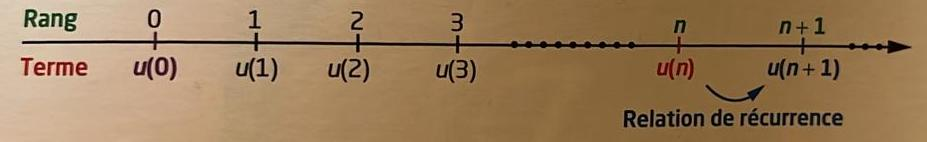
\includegraphics[width=0.9\linewidth]{schema_suites.jpeg}
    \caption{\label{} Suite}
  \end{figure}
}{\vspace{2em}}
\end{tcolorbox}

\textbf{Exemples} \par
\vspace{0.5em}
$u = \left\{15, -3, 7, 8, 97, ...\right\}$ est une suite. \par 
En faisant commencer l'indice de la suite à 0, le terme d'indice 4, noté $u(4)$ est égal à \trou{\textcolor{blue}{8}}{\ndots[3]} \par 
\trou{\[
u(4) = 8
\]}{\vspace{2em}}

\vspace{1em}

Dans certains cas on comptera les positions à partir de 0, dans d'autres à partir de 1 (l'énoncé dira quelle convention utiliser). \par
\vspace{1em}
Par exemple dans la suite $u$ ci-dessus :
\begin{itemize}[noitemsep]
  \item $u(2)= \trou{-3}{\ndots[4]}$ si on compte les positions à partir de 1,
  \item $u(2)= \trou{7}{\ndots[4]}$ si on compte les positions à partir de 0.
\end{itemize}

Si l'énoncé dit "pour tout entier naturel $n$" ou "pour $n \in \mathbb{N}$" , cela voudra dire que l'on compte à partir de 0.
De façon générale, on peut commencer notre suite à n'importe quel rang $n \geq 0$.

\subsection*{Exemples}

Soit $v$ la suite des nombres impairs. Donner $v(5)$ en supposant que les indices débutent à 0. \par
\vspace{1em}
\trou{
  Réponse: $v = \{1;3;5;7;9;11;...\}$, d'où $v(5) = 11$.
}
{\vspace{2em}}


\begin{tcolorbox}[colback=blue!10!white, colframe=blue!75!black, title=Exercices]
  Exercices 1, 3, 5, 6
\end{tcolorbox}

\section*{Représentation graphique d'une suite}
\vspace{1em}

La représentation graphique d'une suite $u$ sera un nuage de points. Ces points auront pour coordonnées $(n ; U_n)$.
En reprenant l'exemple de la suite u des multiples de 2, la représentation graphique de u est :

\trou{
  \begin{figure}[H]
    \centering
    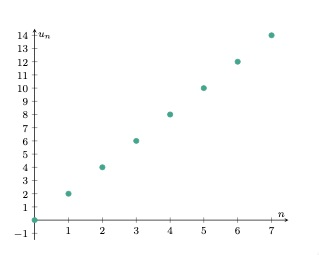
\includegraphics[width=0.5\linewidth]{representation_graphique.jpg}
    \caption{\label{} Représentation graphique}
  \end{figure}
}
{\vspace{7em}}

\section*{Suite définie comme une fonction}
\vspace{1em}

Plutôt que de donner chacun des termes d'une suite, on peut la définir à l'aide d'une formule. La première façon de définir une suite est à l'aide d'une \trou{\textbf{fonction du rang n}}{\ndots[20]}.
On dit que la suite est définie \trou{\textbf{de façon explicite / fonctionnelle.}}{\ndots[20]}

\begin{tcolorbox}[colback=blue!10!white, colframe=blue!75!black, title=Exercices]
  Soit $u$ la suite définie pour tout entier naturel $n$ par $u(n) = 2n - 3$. \par 
  On trouve chaque terme de la suite en remplaçant $n$ par 0,puis 1, 2, etc.
  Ainsi $u(10) = 2 \times 10 - 3 = 17$ et de façon plus générale $u = { \trou{\{-3 ; -1 ; 3; 3 ; ...\}}{\ndots[20]}}$. \par
  \vspace{1em}
  Représenter graphiquement la suite $U$
  \vspace{6em}
\end{tcolorbox}

C'est comme si on échantillonait une fonction (c'est-à-dire qu'on ne sélectionnait les valeurs que pour des valeurs de $x$ données (des nombres entiers))

\begin{figure}[H]
  \centering
  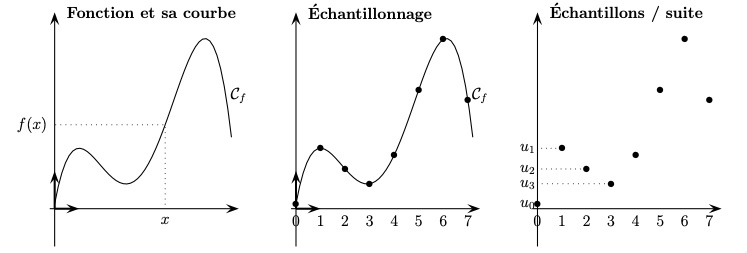
\includegraphics[width=0.8\linewidth]{echantillonage.jpg}
  \caption{\label{} Echantillonage}
\end{figure}

\begin{tcolorbox}[colback=blue!10!white, colframe=blue!75!black, title=Exercices]
  On considère la suite $U(n) = n^2$. Donner les 4 premiers termes de la suite en commençant à $n = 0$

  \trou{
    \[
    \left\{
      \begin{array}{ll}
            U(0) = 0 \\
            U(1) = 1^2 = 1 \\
            U(2) = 2^2 = 4 \\
            U(3) = 3^2 = 9 \\
        \end{array}
      \right.
    \]
  }{\vspace{5em}}

\end{tcolorbox}

\section*{Expression de $U_{N-1}$, $U_{N+1}$, $U_{2N}$, ...}

Si l'expression de $U_n$ est donnée, on peut donner celle de $U_{n+1}$ en remplaçant $n$ par $n + 1$ (en n'oubliant pas les parenthèses).
De même on peut donner l'expression de $U_{2n}$ en remplaçant $n$ par $2n$. \par
\vspace{1em}
\textcolor{blue}{Exemple} : Soit la suite $u$ définie pour tout entier naturel par
\[
  U_n = 7n + 5
\] \par

Donner l'expression de $U_{n+1}$ et de $U_{2n}$

\trou{\vspace{5em}}{\vspace{5em}}

\begin{tcolorbox}[colback=blue!10!white, colframe=blue!75!black, title=Exercices]
  Exercice N°17 page 123 et Question 2 de Exercice N°19
\end{tcolorbox}

\section*{Suite définie par récurrence}

\textbf{Préambule}
\vspace{1em}
Pour maîtriser la partie qui suit, il est nécessaire de comprendre que : 
\begin{itemize}[noitemsep]
    \item $u(n+1)$ est le terme après $u(n)$,
    \item $u(n)$ est le terme après $u(n-1)$,
    \item $u(n-1)$ est le terme après $u(n-2)$,
    \item etc.
\end{itemize}

Et aussi que :
\begin{itemize}[noitemsep]
    \item si $u(n+1)$ est $u(4)$, alors $u(n)$ est $u(3)$,
    \item si $u(n+1)$ est $u(12)$, alors $u(n)$ est $u(11)$,
    \item si $u(n)$ est $u(10)$, alors $u(n-1)$ est $u(9)$.
\end{itemize}


La seconde façon de définir une suite est par récurrence. Dans ce cas, pour calculer la valeur d'un terme de la suite, on a besoin d'un ou plusieurs termes précédents. Ainsi, on aura par exemple une formule du type :
\[
u_{n+1} = \ldots u_n \ldots
\]
ou
\[
u_n = \ldots u_{n-1} \ldots
\]

\begin{tcolorbox}[colback=blue!10!white, colframe=blue!75!black, title=Exercices]

  Soit la suite définie comme suit : 

  \[
    \left\{
      \begin{array}{ll}
            u(n+1) = 4 u(n) + 7 \\
            u(0) = -1 
        \end{array}
      \right.
    \]

  Calculer $u(1)$ et $u(2)$

  \trou{
  Pour calculer $u_1$
  \[
  u(1) = 4u(0) + 7 = 4 \times (-1) + 7 = 3
\]
  Maintenant que l'on connaît $u_1$, on peut calculer $u_2$ : \\
  \[
  u(2) = 4u(1) + 7 = 4 \times 3 + 7 = 19
  \]

  }
  {\vspace{6em}}
  \textbf{Faire l'exercice 66. Conjecturer le sens de variation}
\end{tcolorbox}

\section*{Sens de variation}

\begin{itemize}
\item Une suite est \textbf{croissante} si un terme de la suite est toujours plus grand que son précédent : 
\[
u(n + 1) \geq u(n), \quad \text{pour tout } n \in \mathbb{N}.
\]

\item Une suite est \textbf{décroissante} si : 
\[
u(n + 1) \leq u(n), \quad \text{pour tout } n \in \mathbb{N}.
\]
\end{itemize}

\section*{Définition d'une suite arithmétique}

Une suite est dite \textit{arithmétique} lorsque l'on passe d'un terme au suivant en ajoutant toujours le même nombre. Ainsi, pour tout $n$ :

\[
u(n + 1) = u(n) + r
\]

Le nombre $r$ est appelé \textit{raison} de la suite arithmétique.

\subsubsection*{Exemples}

\begin{itemize}[noitemsep]
    \item La suite définie par $u(n + 1) = u(n) + 4$ est une suite arithmétique de raison 4.
    \item La suite définie par $u(n) = u(n - 1) + 12$ est une suite arithmétique de raison 12.
\end{itemize}

\subsubsection*{Monotonie / Sens de variation}

\begin{itemize}[noitemsep]
    \item Si $r > 0$, la suite est strictement croissante.
    \item Si $r < 0$, la suite est strictement décroissante.
    \item Si $r = 0$, la suite est constante.
\end{itemize}

\subsubsection*{Exemple}

La suite définie par $u(n + 1) = u(n) - 4$ est une suite décroissante.

\subsection*{Reconnaître une suite arithmétique}

\subsubsection*{Suite définie explicitement}

Une suite donnée sous forme explicite peut être une suite arithmétique. Par exemple, la suite $(u_n)$ définie pour tout entier naturel $n$ par :

\[
u(n) = n + 4
\]

est une suite arithmétique. Comment le prouver ?

\begin{enumerate}[noitemsep]
    \item Exprimer $u(n + 1)$.
    \item Calculer $u(n + 1) - u(n)$.
    \item Si le résultat est une constante, c'est-à-dire s'il ne dépend pas de la variable $n$, alors la suite est arithmétique.
\end{enumerate}

\trou{
\vspace{1em}
\textbf{Réponses}

\begin{enumerate}[noitemsep]
    \item $u(n + 1) = (n + 1) + 4 = n + 1 + 4 = n + 5$
    \item $u(n + 1) - u(n) = (n + 5) - (n + 4) = n + 5 - n - 4 = 1$
    \item Comme le résultat de $u(n + 1) - u(n)$ est une constante ($1$), la suite est arithmétique de raison $1$.
\end{enumerate}

On peut donc réécrire $u$ sous la forme :

\[
u(n + 1) = u(n) + 1
\]
}
{\vspace{6em}}

\begin{tcolorbox}[colback=blue!10!white, colframe=blue!75!black, title=Exercices]
  Exercice N°89, N°95, N°97, N°100 page 129-130
\end{tcolorbox}

\section*{Définition d'une suite géométrique}

\begin{tcolorbox}[colback=green!5!white, colframe=green!75!black, title=\textbf{Définition}]
  On dit qu'une suite est \textbf{géométrique} quand on passe d'un terme au suivant en multipliant toujours par le même nombre. Ainsi, pour tout $n$ :
  \[
  u(n+1) = u(n) \times q
  \]
  On appelle ce nombre $q$ la \textbf{raison} de la suite géométrique.
  \end{tcolorbox}
  
\subsection*{Exemples}

  \begin{itemize}[noitemsep]
      \item La suite $u(n+1) = u(n) \times 7$ est une suite géométrique dont la raison est 7.
      \item La suite $u(n) = -6 \times u(n-1)$ est une suite géométrique dont la raison est $-6$.
  \end{itemize}

  \subsection*{Monotonie}  

  \begin{itemize}[noitemsep]
      \item Si $q > 1$, la suite est strictement croissante.
      \item Si $0 < q < 1$, la suite est strictement décroissante.
  \end{itemize}
  
  \subsection*{Autres exemples}

  La suite $u$ définie par tout entier naturel par $u(n+1) = 5u(n)$ est une suite croissante. \par
  La suite $v$ définie par tout entier naturel par $v(n+1) = \frac{1}{2} v(n)$ est une suite décroissante. \par
  
  \vspace{1em}
  Une suite donnée sous forme explicite peut être une suite géométrique. Par exemple, la suite $(u_n)$ définie pour tout entier naturel $n$ par $u(n) = 4^n$ est une suite géométrique. \\
  Comment le prouver ?
  \vspace{1em}
  \begin{enumerate}[noitemsep]
      \item Exprimer $u(n+1)$.
      \item Calculer $\frac{u(n+1)}{u(n)}$.
      \item Si le résultat est une constante, alors la suite est géométrique.
  \end{enumerate}
  
  

  Montrons que la suite $(u_n)$ définie pour tout entier naturel $n$ par $u(n) = 4^n$ est une suite géométrique.
  \[
  \frac{u(n+1)}{u(n)} = \frac{4^{n+1}}{4^n} = 4^{n+1 - n} = 4^1 = 4.
  \]
  Comme le résultat de $\frac{u(n+1)}{u(n)}$ est une constante (4), la suite est géométrique de raison 4. On peut donc réécrire $u$ sous la forme :
  \[
  u(n+1) = 4 \cdot u(n).
  \]
  

\end{document}
